

\tikzset{every picture/.style={line width=0.75pt}} %set default line width to 0.75pt        

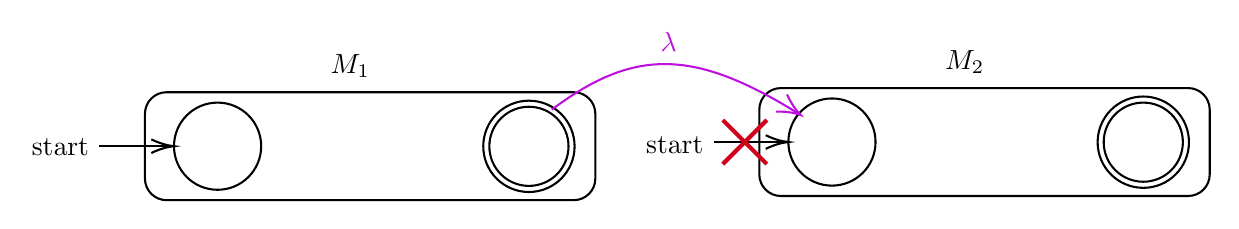
\begin{tikzpicture}[x=0.75pt,y=0.75pt,yscale=-1,xscale=1]
%uncomment if require: \path (0,300); %set diagram left start at 0, and has height of 300

%Straight Lines [id:da648531735118129] 
\draw    (84,145) -- (118,145) ;
\draw [shift={(120,145)}, rotate = 180] [color={rgb, 255:red, 0; green, 0; blue, 0 }  ][line width=0.75]    (10.93,-3.29) .. controls (6.95,-1.4) and (3.31,-0.3) .. (0,0) .. controls (3.31,0.3) and (6.95,1.4) .. (10.93,3.29)   ;
%Shape: Circle [id:dp664310839398671] 
\draw   (120,145) .. controls (120,133.4) and (129.4,124) .. (141,124) .. controls (152.6,124) and (162,133.4) .. (162,145) .. controls (162,156.6) and (152.6,166) .. (141,166) .. controls (129.4,166) and (120,156.6) .. (120,145) -- cycle ;
%Shape: Donut [id:dp6384828907429212] 
\draw   (271.93,145.07) .. controls (271.93,134.54) and (280.47,126) .. (291,126) .. controls (301.53,126) and (310.07,134.54) .. (310.07,145.07) .. controls (310.07,155.6) and (301.53,164.13) .. (291,164.13) .. controls (280.47,164.13) and (271.93,155.6) .. (271.93,145.07)(269,145.07) .. controls (269,132.92) and (278.85,123.07) .. (291,123.07) .. controls (303.15,123.07) and (313,132.92) .. (313,145.07) .. controls (313,157.22) and (303.15,167.07) .. (291,167.07) .. controls (278.85,167.07) and (269,157.22) .. (269,145.07) ;
%Rounded Rect [id:dp6107834080459227] 
\draw   (106,129.4) .. controls (106,123.66) and (110.66,119) .. (116.4,119) -- (312.6,119) .. controls (318.34,119) and (323,123.66) .. (323,129.4) -- (323,160.6) .. controls (323,166.34) and (318.34,171) .. (312.6,171) -- (116.4,171) .. controls (110.66,171) and (106,166.34) .. (106,160.6) -- cycle ;
%Straight Lines [id:da7769953635464104] 
\draw    (380,143) -- (414,143) ;
\draw [shift={(416,143)}, rotate = 180] [color={rgb, 255:red, 0; green, 0; blue, 0 }  ][line width=0.75]    (10.93,-3.29) .. controls (6.95,-1.4) and (3.31,-0.3) .. (0,0) .. controls (3.31,0.3) and (6.95,1.4) .. (10.93,3.29)   ;
%Shape: Circle [id:dp24242726181846175] 
\draw   (416,143) .. controls (416,131.4) and (425.4,122) .. (437,122) .. controls (448.6,122) and (458,131.4) .. (458,143) .. controls (458,154.6) and (448.6,164) .. (437,164) .. controls (425.4,164) and (416,154.6) .. (416,143) -- cycle ;
%Shape: Donut [id:dp17156443887009476] 
\draw   (567.93,143.07) .. controls (567.93,132.54) and (576.47,124) .. (587,124) .. controls (597.53,124) and (606.07,132.54) .. (606.07,143.07) .. controls (606.07,153.6) and (597.53,162.13) .. (587,162.13) .. controls (576.47,162.13) and (567.93,153.6) .. (567.93,143.07)(565,143.07) .. controls (565,130.92) and (574.85,121.07) .. (587,121.07) .. controls (599.15,121.07) and (609,130.92) .. (609,143.07) .. controls (609,155.22) and (599.15,165.07) .. (587,165.07) .. controls (574.85,165.07) and (565,155.22) .. (565,143.07) ;
%Rounded Rect [id:dp6007686314112617] 
\draw   (402,127.4) .. controls (402,121.66) and (406.66,117) .. (412.4,117) -- (608.6,117) .. controls (614.34,117) and (619,121.66) .. (619,127.4) -- (619,158.6) .. controls (619,164.34) and (614.34,169) .. (608.6,169) -- (412.4,169) .. controls (406.66,169) and (402,164.34) .. (402,158.6) -- cycle ;
%Curve Lines [id:da3322917865026447] 
\draw [color={rgb, 255:red, 189; green, 16; blue, 224 }  ,draw opacity=1 ]   (302,127.4) .. controls (341.6,97.7) and (370.42,97.99) .. (420.48,129.05) ;
\draw [shift={(422,130)}, rotate = 212.11] [color={rgb, 255:red, 189; green, 16; blue, 224 }  ,draw opacity=1 ][line width=0.75]    (10.93,-4.9) .. controls (6.95,-2.3) and (3.31,-0.67) .. (0,0) .. controls (3.31,0.67) and (6.95,2.3) .. (10.93,4.9)   ;
\draw  [color={rgb, 255:red, 208; green, 2; blue, 27 }  ,draw opacity=1 ][line width=1.5]  (384.39,132.39) -- (405.61,153.61)(405.61,132.39) -- (384.39,153.61) ;

% Text Node
\draw (50,140) node [anchor=north west][inner sep=0.75pt]   [align=left] {start};
% Text Node
\draw (194,99.4) node [anchor=north west][inner sep=0.75pt]    {$M_{1}$};
% Text Node
\draw (346,139) node [anchor=north west][inner sep=0.75pt]   [align=left] {start};
% Text Node
\draw (490,97.4) node [anchor=north west][inner sep=0.75pt]    {$M_{2}$};
% Text Node
\draw (353,88.4) node [anchor=north west][inner sep=0.75pt]    {$\textcolor[rgb]{0.74,0.06,0.88}{\lambda }$};


\end{tikzpicture}